\section{Methodology}
In this report, a Genetic Algorithm (GA) is explored to solve the QAP. Each individual in the initial population is constructed using the MIP model presented above. Since the solution space is so large and the set of feasible solutions is comparitavely small, starting with an initial set of feasible solutions is useful in guiding the algorithm towards feasibility. Crucial aspects of a GA are selection and reproduction. Elite selection of individuals who survive and reproduce is implemented. One parent is selected from a set of elite individuals, who have an objective value in the top 25\% of the whole population, and the other parent is selected from the whole population. To produce offspring, the simple to implement and computationally inexpensive, round crossover operator is implemented. First, a crossover round is randomly selected. Two children are produced: the first child inherits all rounds up to the cross-over round from the elite parent and the rest of the fixture from the non-elite parent; the second child inherits all rounds up to the cross-over round from the non-elite parent and the rest of the rounds are inherited from the elite parent. Now, we have two parent fixtures and two children fixtures. Of them, the fixture with the worst objective value is removed from the population. After a specified timeframe, the best fixture in the population is taken. 

\bigskip
The steps in the Genetic Algorithm are presented in Figure \ref{fig:flowchart}. First, an initial population is constructed using the MIP model. For a specified period of time, the population evolves. Evolution consists of the following steps: (1) Two parents are selected with one parent being selected from a pool of elite individuals; (2) The two parents are combined through a crossover operator to produce a child; and (3) The family member with the worst objective value is removed. 

\begin{figure}[H]
    \centering
    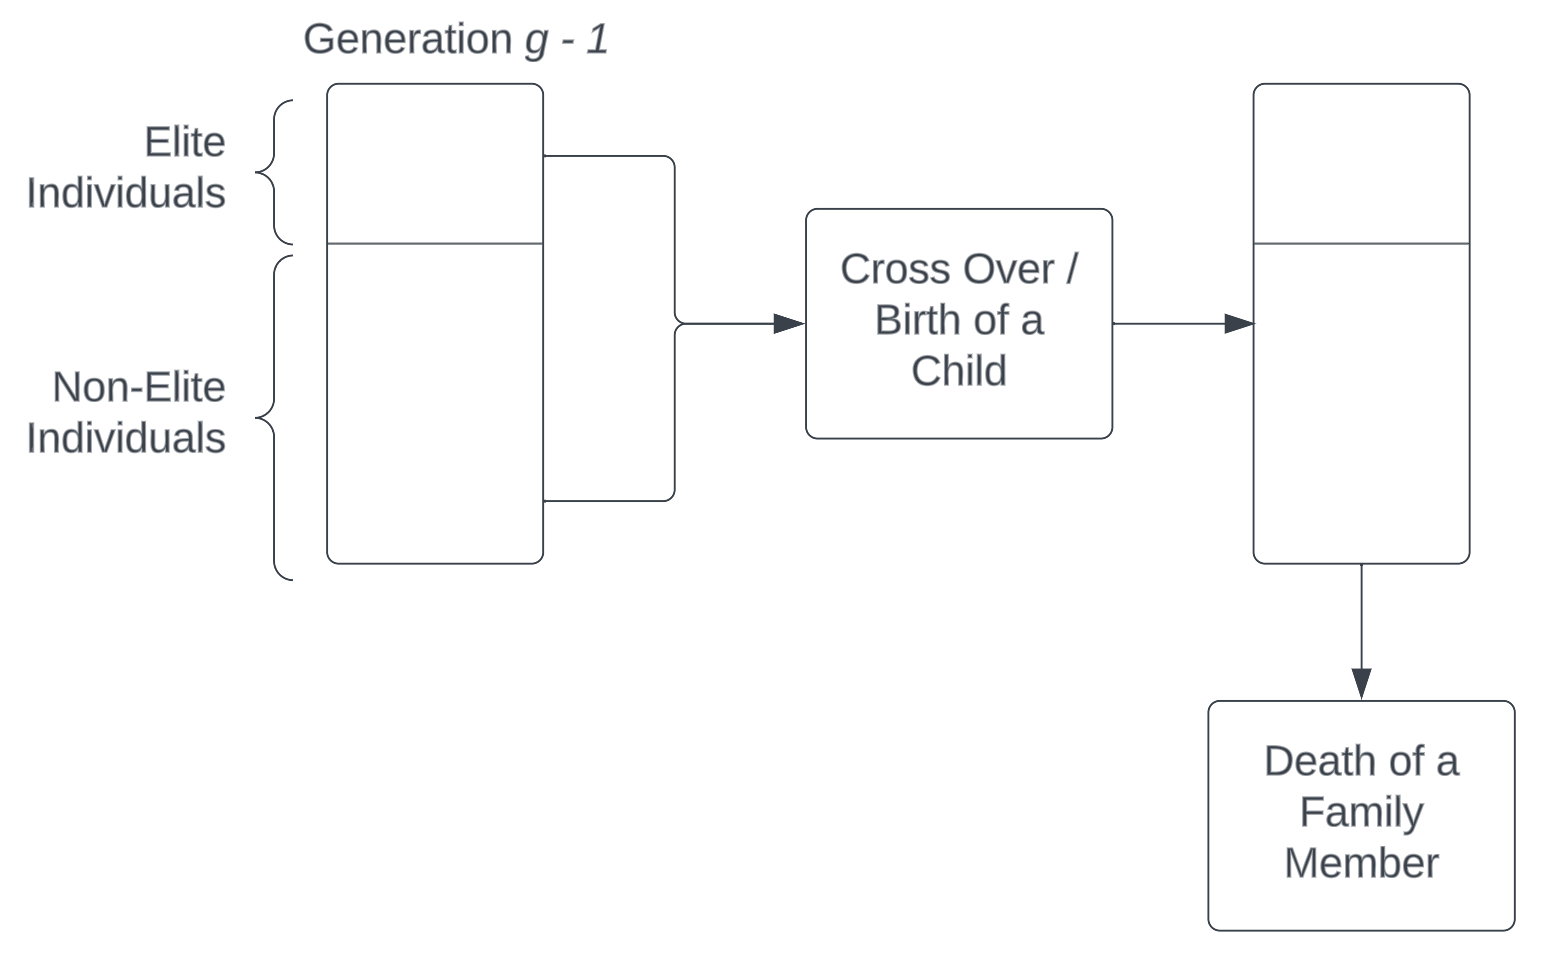
\includegraphics[width=\textwidth]{Figures/GA_flowchart.png}
    \caption{Flow of the Genetic Algorithm}
    \label{fig:flowchart}
\end{figure}

